\documentclass{standalone}
\usepackage[rgb]{xcolor}
\usepackage{tikz}
\usetikzlibrary{through}

\begin{document}
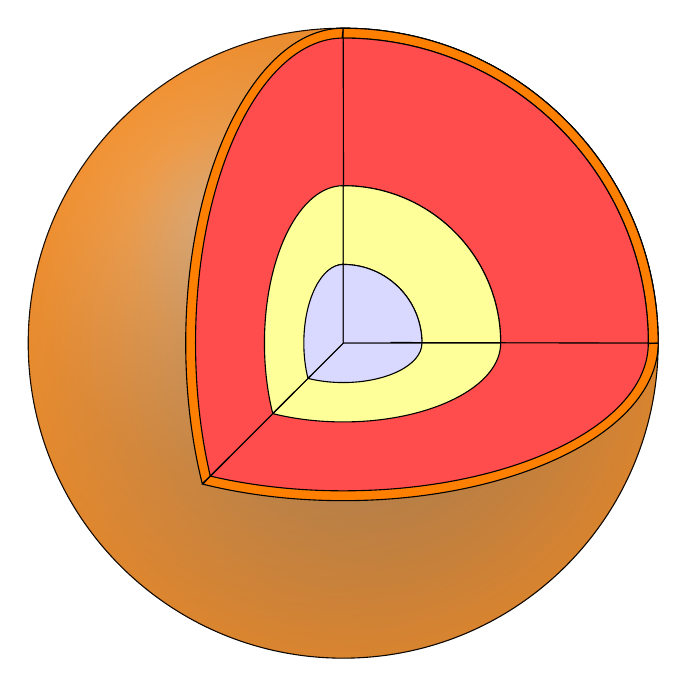
\begin{tikzpicture}[inner sep=0, outer sep=0]
    % coordinaten
    \coordinate (m) at (0,4,0);
    % assen
    \draw  (0,0,0) -- (0,4,0); % z
    \draw  (0,0,0) -- (4,0,0); % x
    \draw  (0,0,0) -- (0,0,4.65); % y
    % sfeer
    \draw (4,0,0) arc (0:116.5:4cm and -2cm);
    \draw (4,0,0) arc (0:90:4cm and 4cm);
    \draw (0,4,0) arc (90:206.5:2cm and 4cm);
    \node[draw, inner color=black!50, outer color=orange!75, circle 
through={(m)}] (c) at (0,0,0) {};
    \node [ball color=orange, fill opacity=.25, circle through={(m)}] at 
(0,0,0) {};
    % fotosfeer
    \draw (3.875,0,0) arc (0:115.8:3.875cm and -1.875cm);
    \draw (3.875,0,0) arc (0:90:3.875cm and 3.875cm);
    \draw (0,3.875,0) arc (90:205.8:1.875cm and 3.875cm);
    % convenctie zone
    \draw (2,0,0) arc (0:116.5:2cm and -1cm);
    \draw (2,0,0) arc (0:90:2cm and 2cm);
    \draw (0,2,0) arc (90:206.5:1cm and 2cm);
    % radiatie zone
    \draw (1,0,0) arc (0:116.5:1cm and -0.5cm);
    \draw (1,0,0) arc (0:90:1cm and 1cm);
    \draw (0,1,0) arc (90:206.5:0.5cm and 1cm);
    % fill
    \draw[fill=orange] (4,0,0) arc (0:90:4cm and 4cm) -- (0,3.875,0) arc 
(90:0:3.875cm and 3.875cm) -- (4,0,0);
    \draw[fill=red!70] (3.875,0,0) arc (0:90:3.875cm and 3.875cm) -- (0,2,0) 
arc (90:0:2cm and 2cm) -- (3.875,0,0);
    \draw[fill=yellow!40] (2,0,0) arc (0:90:2cm and 2cm) -- (0,1,0) arc 
(90:0:1cm and 1cm) -- (2,0,0);
    \draw[fill=blue!15] (1,0,0) arc (0:90:1cm and 1cm) -- (0,0,0) -- (1,0,0);
    \draw[fill=orange] (4,0,0) arc (0:116.5:4cm and -2cm) -- (0,0,3.875) arc 
(115.8:0:3.7cm and -1.65cm) -- (4,0,0);
    \draw[fill=red!70] (3.875,0,0) arc (0:115.8:3.875cm and -1.875cm) -- 
(0,0,2) arc (115.8:0:.96cm and -.865cm) -- (3.875,0,0);
    \draw[fill=yellow!40] (2,0,0) arc (0:116.5:2cm and -1cm) -- (0,0,1) arc 
(115.8:0:.96cm and -.43cm) -- (2,0,0);
    \draw[fill=blue!15] (1,0,0) arc (0:116.5:1cm and -.5cm) -- (0,0,0) -- 
(1,0,0);
    \draw[fill=orange] (0,4,0) arc (90:206.5:2cm and 4cm) -- (0,0,3.875) arc 
(206.5:90:1.65cm and 3.7cm) -- (0,4,0);
    \draw[fill=red!70] (0,3.875,0) arc (90:205.8:1.875cm and 3.875cm) -- 
(0,0,2) arc (205.8:90:.86cm and 1.925cm) -- (0,3.875,0);
    \draw[fill=yellow!40] (0,2,0) arc (90:206.5:1cm and 2cm) -- (0,0,1) arc 
(206.5:90:.43cm and .96cm) -- (0,2,0);
    \draw[fill=blue!15] (0,1,0) arc (90:206.5:.5cm and 1cm) -- (0,0,0) -- 
(0,1,0);
\end{tikzpicture}
\end{document}
